\subsection{FP8 Quantization}
\label{section:fp8}
We perform experiments leveraging the native FP8 support of H100 GPUs to perform low-precision inference.
To enable low-precision inference, we apply FP8 quantization to most matrix multiplications inside the model.
In particular, we quantize most parameters and activations in the feedforward network layers in the model, which account for roughly 50\% of the inference compute time.
We do not quantize parameters in the self-attention layers of the model.
We leverage dynamic scaling factors for better accuracy~\citep{xiao2024smoothquant}, optimizing our CUDA kernels\footnote{Our FP8 kernels are available at \url{https://github.com/pytorch/FBGEMM/tree/main/fbgemm_gpu/experimental/gen_ai}. We provide usage examples at \url{https://github.com/meta-llama/llama-agentic-system}.} to reduce the overhead of calculating the scales.
We find that the quality of \llamathree 405B is sensitive to certain types of quantization, and make a few additional changes to increase the model output quality:

\begin{enumerate}
    \item Akin to \cite{zhang2021training}, we do not perform quantization in the first and last Transformer layers.
    \item High-perplexity tokens such as dates can lead to large activation values. In turn, these can lead to high dynamic scaling factors in FP8 and a non-negligible number of underflows, leading to errors in decoding. To address this issue, we upper bound the dynamic scaling factors to $1200$.
    \item We use row-wise quantization, computing scaling factors across rows for  parameter and activation matrices (see Figure~\ref{figure:fp8-schematic}). We find this works better than a tensor-wise quantization approach. 
\end{enumerate}

\begin{figure}[t]
\hspace*{-1.2cm}   
\centering
\includegraphics[scale=0.3]{assets/llama3-figure-25.eps}
\caption{\textbf{Illustration of tensor-wise and row-wise FP8 quantization.} \emph{Right:} Row-wise quantization enables the use of more granular activation factors than \emph{Left:} tensor-wise quantization.}
\label{figure:fp8-schematic}
\end{figure}

\textbf{Effect of quantization errors.} Evaluations on standard benchmarks often suggest that FP8 inference performs on par with BF16 inference even without these mitigations.
However, we find that such benchmarks do not adequately reflect the effects of FP8 quantization.
When scaling factors are not upper bounded, the model occasionally produces corrupted responses even though the benchmark performance is strong.
Instead of relying on benchmarks to measure distribution changes due to quantization, we find it is better to analyze the distribution of reward-model scores for $100,000$ responses produced using both FP8 and BF16.
Figure \ref{figure:reward-scores} shows the resulting reward distribution for our quantization approach.
The results in the figure show that our approach to FP8 quantization has very limited impact on the model's response. 

\begin{figure}[t]
\centering
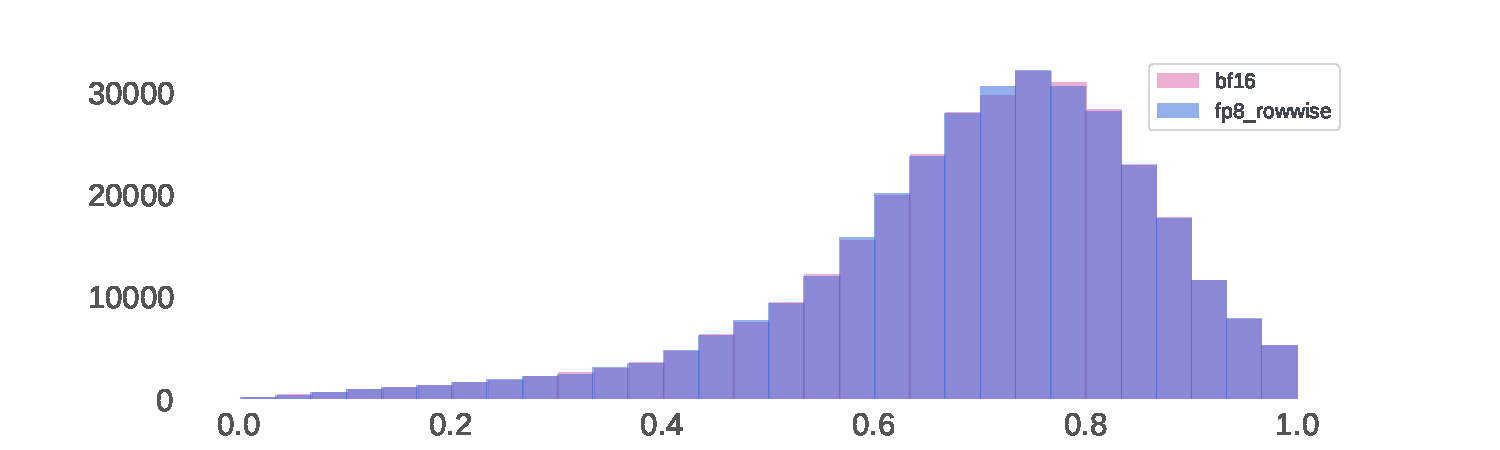
\includegraphics[scale=0.5]{assets/bf16_vs_fp8_new.pdf}
\caption{\textbf{Reward score distribution for Llama 3 405B using BF16 and FP8 inference.} Our FP8 quantization approach has negligible impact on the model's responses.}
\label{figure:reward-scores}
\end{figure}

\textbf{Experimental evaluation of efficiency.}
Figure~\ref{figure:fp8_speed} depicts the throughput-latency trade-off of performing FP8 inference with \llamathree 405B in the pre-fill and decoding stages, using 4,096 input tokens and 256 output tokens.
The figure compares the efficiency of FP8 inference with that of the two-machine BF16 inference approach described in Section~\ref{section:pp}.
The results show that use of FP8 inference leads to throughput improvements of up to 50$\%$ during the pre-fill stage, and a substantially better throughput-latency trade-off during decoding.

\begin{figure}
\centering
  \begin{subfigure}{.5\textwidth}
    \centering
    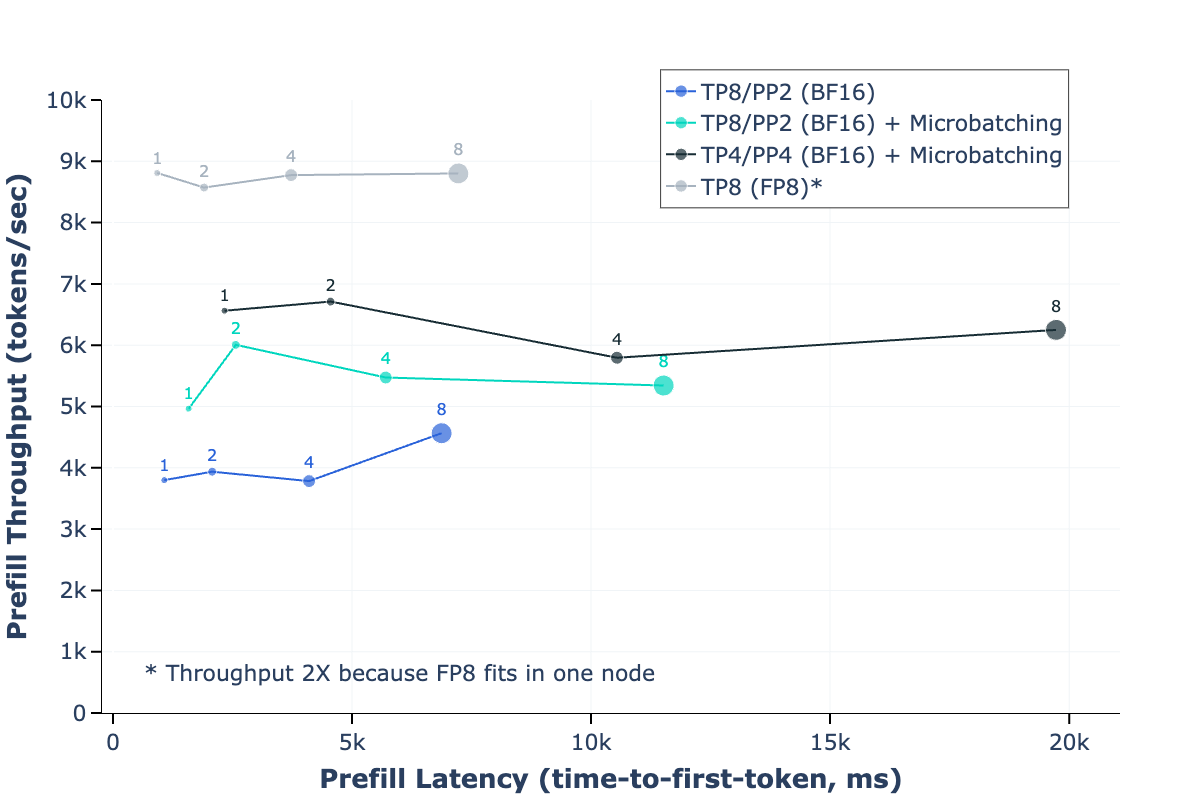
\includegraphics[width=\linewidth]{assets/prefill_fp8.png}
  \end{subfigure}%
  \begin{subfigure}{.5\textwidth}
    \centering
    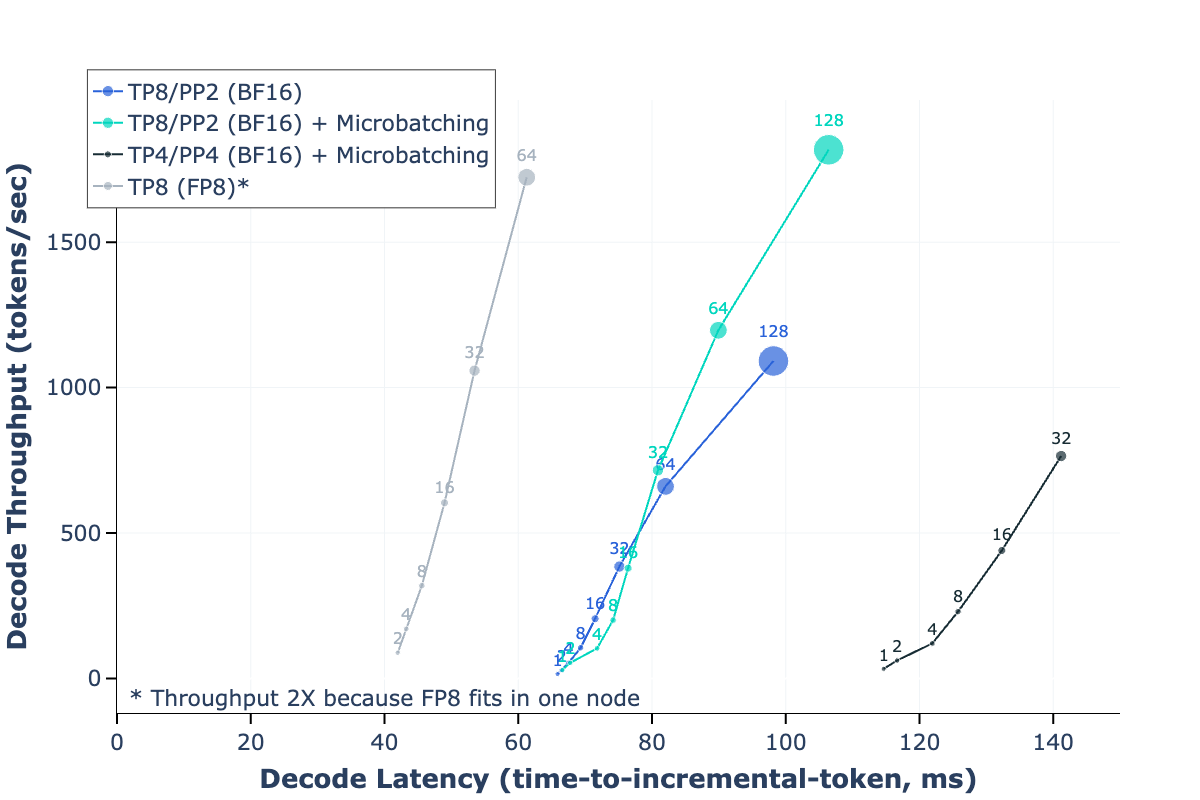
\includegraphics[width=\linewidth]{assets/decode_fp8.png}
  \end{subfigure}
  \caption{\textbf{Throughput-latency trade-off in FP8 inference with Llama 3 405B} compared with BF16 inference using different pipeline parallelization setups. \emph{Left:} Results for pre-filling. \emph{Right:} Results for decoding.}
  \label{figure:fp8_speed}
\end{figure}
